\section{Xây dựng kiến trúc phần mềm cho hệ thống}
\subsection{Module Views}
\subsubsection{Context View}

\begin{figure}[H]
    \centering
    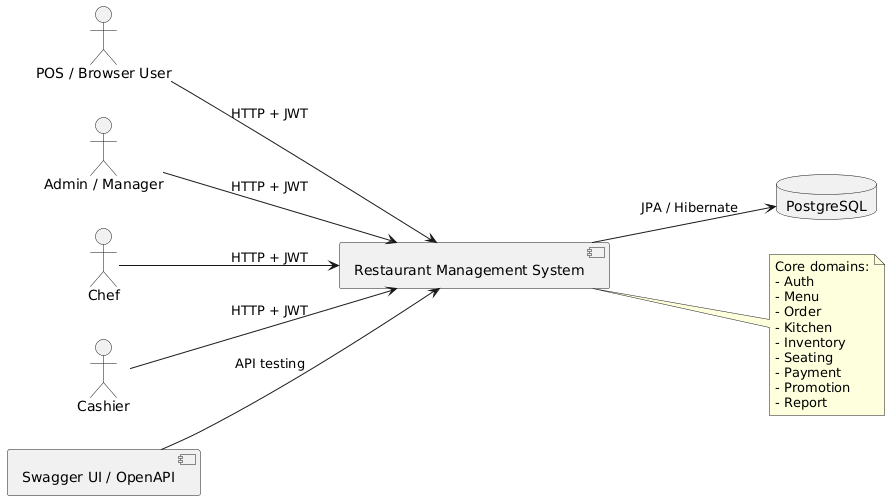
\includegraphics[width=0.95\linewidth]{image/4.1.1.png}
    \caption{Context View của hệ thống}
    \label{fig:context-view}
\end{figure}

Sơ đồ Context View mô tả mối quan hệ tổng quát giữa hệ thống quản lý nhà hàng và các tác nhân bên ngoài. Hệ thống đóng vai trò trung tâm, tiếp nhận yêu cầu từ nhiều nhóm người dùng khác nhau thông qua giao thức HTTP kết hợp cơ chế xác thực JWT.

\textbf{POS / Browser User}: 
Người dùng thông thường sử dụng hệ thống thông qua giao diện POS hoặc trình duyệt web để thực hiện các chức năng như xem thực đơn, đặt món và thanh toán.

\textbf{Admin / Manager}: 
Quản trị viên hoặc quản lý sử dụng hệ thống để quản lý menu, khuyến mãi, báo cáo doanh thu và giám sát hoạt động nhà hàng.

\textbf{Chef}: 
Đầu bếp nhận thông tin đơn hàng từ hệ thống để xử lý và cập nhật trạng thái món ăn.

\textbf{Cashier}: 
Thu ngân sử dụng hệ thống để xử lý thanh toán và xác nhận giao dịch.

\textbf{Restaurant Management System}: 
Là hệ thống trung tâm chứa các domain nghiệp vụ chính bao gồm:
\textit{Auth, Menu, Order, Kitchen, Inventory, Seating, Payment, Promotion, Report}.

\textbf{PostgreSQL}: 
Được sử dụng làm hệ quản trị cơ sở dữ liệu nhằm lưu trữ dữ liệu nghiệp vụ của hệ thống thông qua cơ chế JPA/Hibernate.

\textbf{Swagger UI / OpenAPI}: 
Hỗ trợ kiểm thử và tài liệu hóa RESTful API trong quá trình phát triển và tích hợp hệ thống.

\textbf{Luồng giao tiếp}: 
Người dùng gửi request $\rightarrow$ Restaurant Management System $\rightarrow$ PostgreSQL.

\vspace{0.5cm}

\subsubsection{Package View}

\begin{figure}[H]
    \centering
    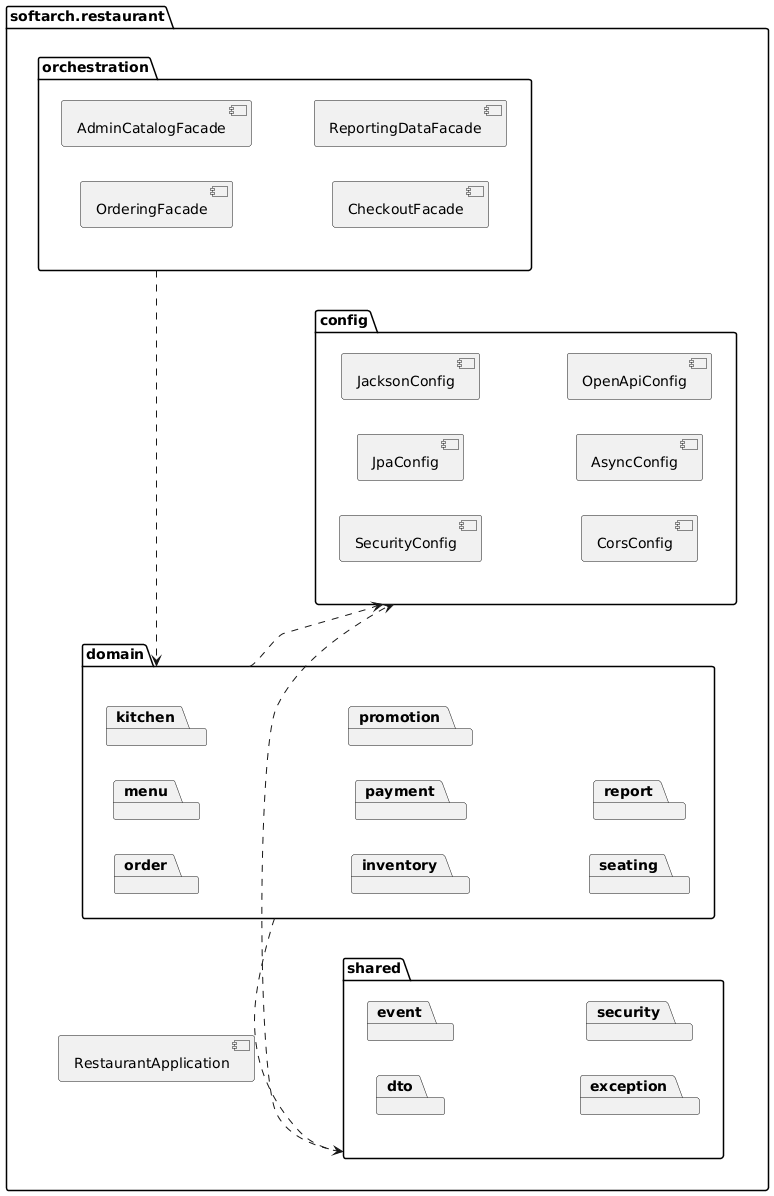
\includegraphics[width=0.7\linewidth]{image/4.1.2.png}
    \caption{Package View của hệ thống}
    \label{fig:package-view}
\end{figure}

Sơ đồ Package View mô tả cấu trúc tổ chức mã nguồn của hệ thống theo các package chức năng nhằm tăng tính phân tách trách nhiệm, khả năng mở rộng và bảo trì.

\textbf{Package config}: 
Chứa các thành phần cấu hình hệ thống như:
\textit{SecurityConfig, JpaConfig, JacksonConfig, CorsConfig, AsyncConfig, OpenApiConfig}. 
Các package này hỗ trợ cấu hình bảo mật, ORM, serialization, CORS, xử lý bất đồng bộ và tài liệu API.

\textbf{Package shared}: 
Chứa các thành phần dùng chung trong toàn hệ thống bao gồm:
\textit{dto, event, exception, security}. 
Các thành phần này giúp tái sử dụng mã nguồn và giảm trùng lặp logic.

\textbf{Package orchestration}: 
Chứa các facade chịu trách nhiệm điều phối luồng nghiệp vụ giữa nhiều domain khác nhau như:
\textit{OrderingFacade, CheckoutFacade, AdminCatalogFacade, ReportingDataFacade}.

\textbf{Package domain}: 
Chứa các domain nghiệp vụ chính của hệ thống:
\textit{order, menu, kitchen, inventory, payment, promotion, seating, report}. 
Mỗi domain được tổ chức độc lập nhằm đảm bảo tính module hóa và giảm coupling giữa các thành phần.

\textbf{RestaurantApplication}: 
Là điểm khởi chạy chính của toàn bộ hệ thống Spring Boot.

\textbf{Quan hệ phụ thuộc}: 
\begin{itemize}
    \item Package \textit{shared} phụ thuộc vào \textit{config} để sử dụng các cấu hình hệ thống.
    \item Package \textit{orchestration} phụ thuộc vào \textit{domain} để điều phối nghiệp vụ.
    \item Package \textit{domain} sử dụng các thành phần dùng chung từ \textit{shared}.
    \item Package \textit{domain} đồng thời phụ thuộc vào \textit{config} cho các cấu hình hạ tầng.
\end{itemize}

\vspace{0.5cm}

\subsubsection{Module View}

\begin{figure}[H]
    \centering
    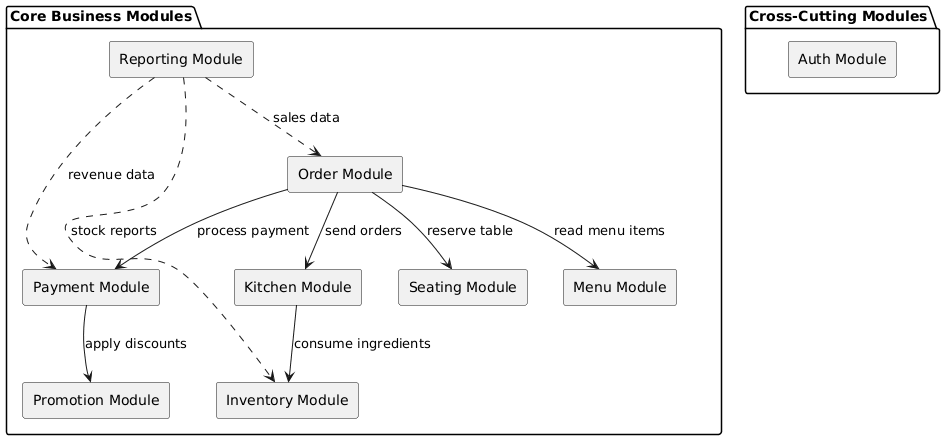
\includegraphics[width=0.9\linewidth]{image/4.1.3.png}
    \caption{Module View của hệ thống}
    \label{fig:module-view}
\end{figure}

Sơ đồ Module View mô tả cấu trúc phân rã hệ thống theo các business module chính nhằm tăng tính độc lập, khả năng mở rộng và tái sử dụng.

Hệ thống được chia thành hai nhóm module chính:

\textbf{Core Business Modules}: 
Bao gồm các module nghiệp vụ cốt lõi của hệ thống:
\begin{itemize}
    \item \textit{Menu Module}: quản lý thực đơn và thông tin món ăn.
    \item \textit{Order Module}: xử lý đặt món và quản lý đơn hàng.
    \item \textit{Kitchen Module}: quản lý hàng chờ chế biến món ăn.
    \item \textit{Payment Module}: xử lý thanh toán và giao dịch.
    \item \textit{Inventory Module}: quản lý nguyên liệu và tồn kho.
    \item \textit{Promotion Module}: quản lý khuyến mãi và giảm giá.
    \item \textit{Seating Module}: quản lý bàn và đặt chỗ.
    \item \textit{Reporting Module}: tổng hợp báo cáo và thống kê doanh thu.
\end{itemize}

\textbf{Cross-Cutting Modules}: 
Bao gồm các module hỗ trợ xuyên suốt toàn hệ thống:
\begin{itemize}
    \item \textit{Auth Module}: cung cấp cơ chế xác thực và phân quyền người dùng thông qua JWT Security.
\end{itemize}

\textbf{Quan hệ giữa các module}:
\begin{itemize}
    \item \textit{Order Module} sử dụng dữ liệu từ \textit{Menu Module} để tạo đơn hàng.
    \item \textit{Order Module} tương tác với \textit{Payment Module} để xử lý thanh toán.
    \item \textit{Order Module} gửi thông tin đơn hàng tới \textit{Kitchen Module}.
    \item \textit{Kitchen Module} cập nhật và tiêu thụ nguyên liệu từ \textit{Inventory Module}.
    \item \textit{Payment Module} áp dụng khuyến mãi từ \textit{Promotion Module}.
    \item \textit{Order Module} tương tác với \textit{Seating Module} để quản lý đặt bàn.
    \item \textit{Reporting Module} thu thập dữ liệu từ các module nghiệp vụ nhằm tạo báo cáo doanh thu, thống kê đơn hàng và tình trạng tồn kho.
\end{itemize}

Sơ đồ Module View giúp mô tả rõ ràng cấu trúc nghiệp vụ của hệ thống và mối quan hệ giữa các business module chính trong kiến trúc phần mềm.


\subsection{Component \& Connector Views}
\subsubsection{Component View}

\begin{figure}[H]
    \centering
    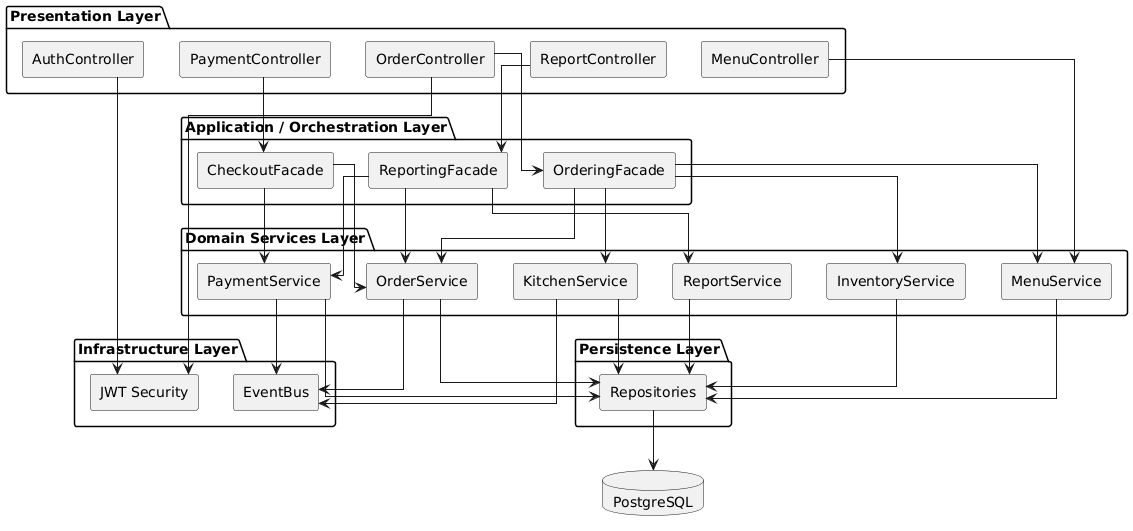
\includegraphics[width=0.95\linewidth]{image/4.2.2.png}
    \caption{Component View của hệ thống}
    \label{fig:component-view}
\end{figure}

Sơ đồ Component View mô tả cấu trúc thành phần bên trong hệ thống và cách các component được tổ chức theo mô hình phân lớp nhằm tăng khả năng mở rộng, tái sử dụng và bảo trì hệ thống.

Khác với Module View chỉ tập trung vào các business module ở mức khái quát, Component View đi sâu hơn vào các thành phần kỹ thuật cụ thể và trách nhiệm của từng component trong hệ thống.

Hệ thống được chia thành các layer chính như sau:

\textbf{Presentation Layer}:  
Bao gồm các controller như:
\textit{AuthController, OrderController, MenuController, PaymentController, ReportController}.  
Các controller đóng vai trò là điểm tiếp nhận HTTP request từ client và chuyển tiếp request tới các lớp xử lý nghiệp vụ tương ứng.

\textbf{Application / Orchestration Layer}:  
Bao gồm các facade như:
\textit{OrderingFacade, CheckoutFacade, ReportingFacade}.  
Lớp này chịu trách nhiệm điều phối các luồng nghiệp vụ phức tạp giữa nhiều domain service khác nhau, giúp giảm coupling giữa Presentation Layer và Domain Layer.

\textbf{Domain Services Layer}:  
Chứa các service nghiệp vụ chính của hệ thống bao gồm:
\textit{OrderService, MenuService, KitchenService, PaymentService, InventoryService, ReportService}.  
Đây là lớp xử lý business logic cốt lõi của hệ thống.

\textbf{Persistence Layer}:  
Bao gồm các repository chịu trách nhiệm truy cập và lưu trữ dữ liệu thông qua JPA/Hibernate.

\textbf{Infrastructure Layer}:  
Bao gồm các thành phần hạ tầng như:
\textit{EventBus} và \textit{JWT Security}.  
Lớp này hỗ trợ xác thực người dùng và giao tiếp bất đồng bộ thông qua cơ chế event-driven.

\textbf{Database}:  
Hệ thống sử dụng PostgreSQL làm cơ sở dữ liệu trung tâm để lưu trữ toàn bộ dữ liệu nghiệp vụ.

\subsubsection*{Luồng hoạt động của Component View}

Quá trình xử lý request trong hệ thống diễn ra theo các bước sau:

\begin{enumerate}
    \item Client gửi HTTP request tới hệ thống.
    
    \item JWT Security thực hiện xác thực và phân quyền request trước khi chuyển tiếp tới controller tương ứng.
    
    \item Controller tiếp nhận request:
    \begin{itemize}
        \item Với các tác vụ đơn giản, controller có thể gọi trực tiếp service.
        \item Với các workflow phức tạp, controller sẽ gọi tới facade để điều phối nghiệp vụ.
    \end{itemize}
    
    \item Facade thực hiện orchestration giữa nhiều domain service khác nhau nhằm xử lý business logic.
    
    \item Domain service thao tác với repository để truy cập hoặc cập nhật dữ liệu trong PostgreSQL.
    
    \item Trong quá trình xử lý, service có thể publish domain events tới EventBus.
    
    \item EventBus thực hiện dispatch event bất đồng bộ tới các listener hoặc service khác nhằm xử lý các tác vụ follow-up.
\end{enumerate}

\subsubsection*{Guideline cho Component View}

Khi xây dựng Component View cho hệ thống, cần tuân thủ các nguyên tắc sau:

\begin{itemize}
    \item Component View phải tập trung mô tả cấu trúc thành phần bên trong hệ thống thay vì business capability ở mức cao.
    
    \item Các component nên được tổ chức theo layer nhằm tăng tính phân tách trách nhiệm (Separation of Concerns).
    
    \item Controller cần giữ vai trò ``thin controller'', chỉ tiếp nhận request và chuyển tiếp xử lý xuống các layer bên dưới.
    
    \item Các workflow nghiệp vụ phức tạp nên được xử lý thông qua facade hoặc orchestration layer để tránh coupling trực tiếp giữa controller và nhiều service.
    
    \item Business logic phải được đặt tại domain services thay vì controller hoặc repository.
    
    \item Repository chỉ chịu trách nhiệm persistence và không chứa business logic.
    
    \item Các thành phần cross-cutting như authentication, event bus hoặc logging nên được tách riêng vào infrastructure layer.
    
    \item Các interaction bất đồng bộ nên được biểu diễn thông qua event-driven connectors như EventBus.
    
    \item Không nên đưa quá nhiều implementation detail vào Component View như entity fields hoặc method-level design vì điều này phù hợp hơn với Class Diagram.
    
    \item Component View cần đảm bảo người đọc có thể nhanh chóng hiểu:
    \begin{itemize}
        \item Hệ thống gồm những component nào.
        \item Vai trò của từng component.
        \item Quan hệ phụ thuộc giữa các component.
        \item Luồng xử lý chính của hệ thống.
    \end{itemize}
\end{itemize}

\subsubsection{Component \& Connector (C\&C) View}

\begin{figure}[H]
    \centering
    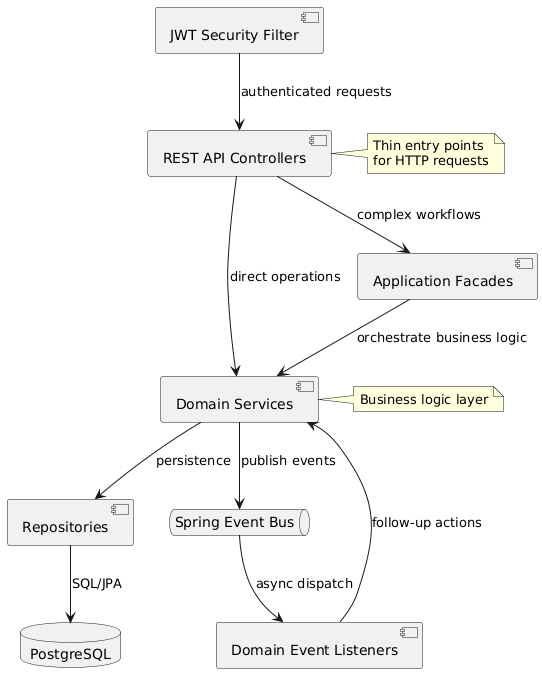
\includegraphics[width=0.9\linewidth]{image/4.2.1.png}
    \caption{Component \& Connector View của hệ thống}
    \label{fig:cc-view}
\end{figure}

Sơ đồ Component \& Connector (C\&C) View mô tả các thành phần runtime của hệ thống và cách các thành phần này giao tiếp với nhau trong quá trình thực thi.

Khác với Component View tập trung vào cấu trúc thành phần, C\&C View tập trung vào:
\begin{itemize}
    \item Runtime interaction.
    \item Luồng xử lý request.
    \item Event-driven communication.
    \item Quan hệ giao tiếp giữa các component.
\end{itemize}

Các thành phần chính trong sơ đồ bao gồm:

\textbf{JWT Security Filter}:  
Thực hiện xác thực và kiểm tra quyền truy cập trước khi request được xử lý bởi hệ thống.

\textbf{REST API Controllers}:  
Tiếp nhận request HTTP từ client và định tuyến request tới các facade hoặc service tương ứng.

\textbf{Application Facades}:  
Điều phối các workflow nghiệp vụ phức tạp giữa nhiều domain service khác nhau.

\textbf{Domain Services}:  
Xử lý business logic chính của hệ thống.

\textbf{Repositories}:  
Thực hiện persistence và truy vấn dữ liệu từ PostgreSQL.

\textbf{Spring Event Bus}:  
Cung cấp cơ chế giao tiếp bất đồng bộ giữa các thành phần thông qua event-driven architecture.

\textbf{Domain Event Listeners}:  
Lắng nghe và xử lý các event được publish từ domain services.

\subsubsection*{Luồng xử lý của C\&C View}

Luồng xử lý runtime của hệ thống được thực hiện như sau:

\begin{enumerate}
    \item Request từ client được xác thực thông qua JWT Security Filter.
    
    \item Request được chuyển tới REST API Controllers.
    
    \item Controller:
    \begin{itemize}
        \item Gọi trực tiếp domain services cho các thao tác đơn giản.
        \item Gọi facade cho các workflow phức tạp cần orchestration.
    \end{itemize}
    
    \item Domain services xử lý business logic và thao tác với repositories để truy cập dữ liệu.
    
    \item Repositories tương tác với PostgreSQL thông qua JPA/Hibernate.
    
    \item Services có thể publish domain events tới Spring Event Bus.
    
    \item EventBus thực hiện dispatch bất đồng bộ tới các listener.
    
    \item Listener thực hiện các tác vụ follow-up hoặc kích hoạt xử lý tiếp theo.
\end{enumerate}

\subsubsection*{Guideline cho C\&C View}

Khi xây dựng C\&C View cần tuân thủ các nguyên tắc sau:

\begin{itemize}
    \item C\&C View phải tập trung vào runtime communication thay vì cấu trúc source code.
    
    \item Chỉ nên mô tả các runtime component quan trọng và các connector chính giữa chúng.
    
    \item Các connector cần thể hiện rõ:
    \begin{itemize}
        \item synchronous communication.
        \item asynchronous communication.
        \item event-driven interaction.
    \end{itemize}
    
    \item Các request flow chính cần được mô tả rõ ràng từ controller tới service và database.
    
    \item Các cơ chế cross-cutting như authentication, messaging hoặc event bus nên được thể hiện rõ trong runtime flow.
    
    \item Không nên đưa quá nhiều chi tiết implementation như entity, DTO hoặc class-level dependency vào C\&C View.
    
    \item Các interaction bất đồng bộ nên được biểu diễn riêng biệt nhằm làm nổi bật kiến trúc event-driven.
    
    \item C\&C View cần giúp người đọc nhanh chóng hiểu:
    \begin{itemize}
        \item Các runtime component chính của hệ thống.
        \item Các connector giữa các component.
        \item Luồng giao tiếp và xử lý request.
        \item Cơ chế giao tiếp đồng bộ và bất đồng bộ.
    \end{itemize}
\end{itemize}


\subsection{Allocation View}

Allocation View mô tả cách hệ thống phần mềm được ánh xạ tới môi trường triển khai, cấu trúc cài đặt và tổ chức nhân sự phát triển hệ thống. View này giúp thể hiện mối quan hệ giữa kiến trúc phần mềm và môi trường thực tế trong quá trình triển khai, vận hành và phát triển hệ thống.

Trong hệ thống quản lý nhà hàng, Allocation View được mô tả thông qua ba góc nhìn chính:
\begin{itemize}
    \item Install Style
    \item Deployment Style
    \item Work Assignment Style
\end{itemize}

\vspace{0.5cm}

\subsubsection{Install Style}

\begin{figure}[H]
    \centering
    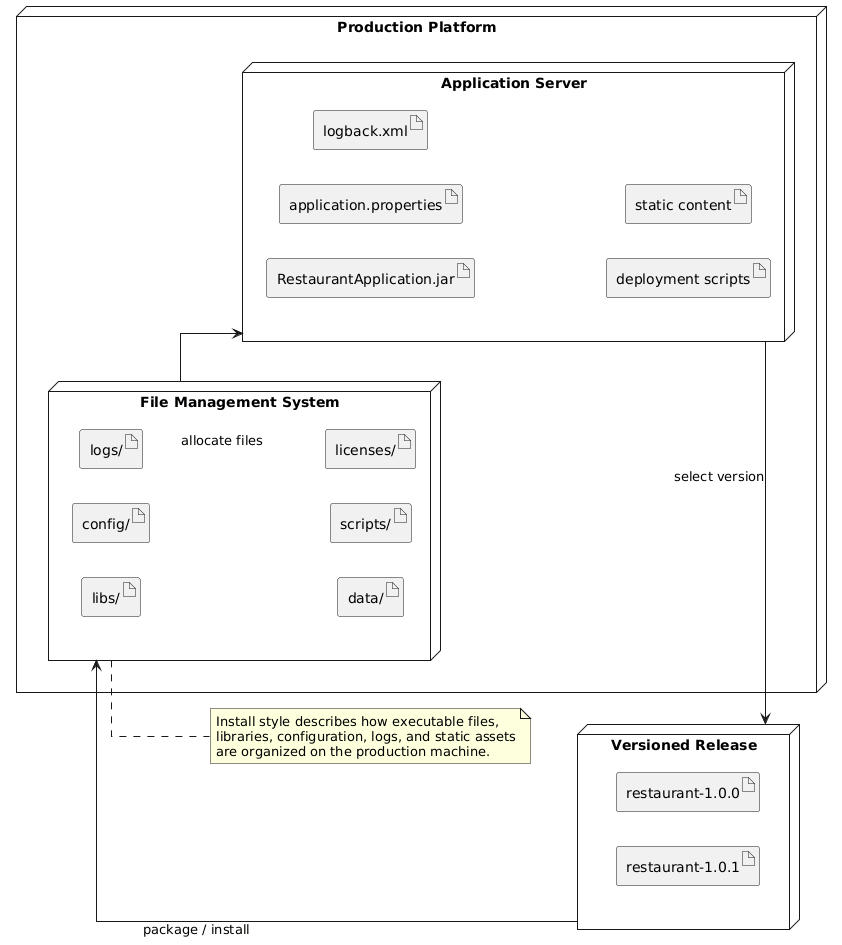
\includegraphics[width=0.9\linewidth]{image/4.3.1.png}
    \caption{Install Style của hệ thống}
    \label{fig:install-style}
\end{figure}

Sơ đồ Install Style mô tả cách các thành phần phần mềm, file cấu hình và tài nguyên hệ thống được tổ chức trên môi trường production.

Hệ thống được triển khai trên một \textit{Production Platform} bao gồm hai thành phần chính:

\textbf{Application Server}:  
Chứa các artifact cần thiết để chạy hệ thống:
\begin{itemize}
    \item \textit{RestaurantApplication.jar}: file thực thi chính của ứng dụng Spring Boot.
    \item \textit{application.properties}: file cấu hình hệ thống.
    \item \textit{logback.xml}: cấu hình logging.
    \item \textit{deployment scripts}: script phục vụ triển khai hệ thống.
    \item \textit{static content}: tài nguyên tĩnh như HTML, CSS, JavaScript và hình ảnh.
\end{itemize}

\textbf{File Management System}:  
Quản lý cấu trúc thư mục và các file cài đặt của hệ thống:
\begin{itemize}
    \item \textit{libs/}: chứa thư viện phụ thuộc.
    \item \textit{config/}: chứa file cấu hình.
    \item \textit{logs/}: chứa log runtime.
    \item \textit{data/}: chứa dữ liệu hệ thống.
    \item \textit{scripts/}: chứa script triển khai và vận hành.
    \item \textit{licenses/}: chứa thông tin giấy phép phần mềm.
\end{itemize}

Ngoài ra, hệ thống còn hỗ trợ quản lý nhiều phiên bản phát hành thông qua các release như:
\textit{restaurant-1.0.0} và \textit{restaurant-1.0.1}.  
Các phiên bản này được package và cài đặt vào môi trường production thông qua File Management System.

\vspace{0.5cm}

\subsubsection{Deployment Style}

\begin{figure}[H]
    \centering
    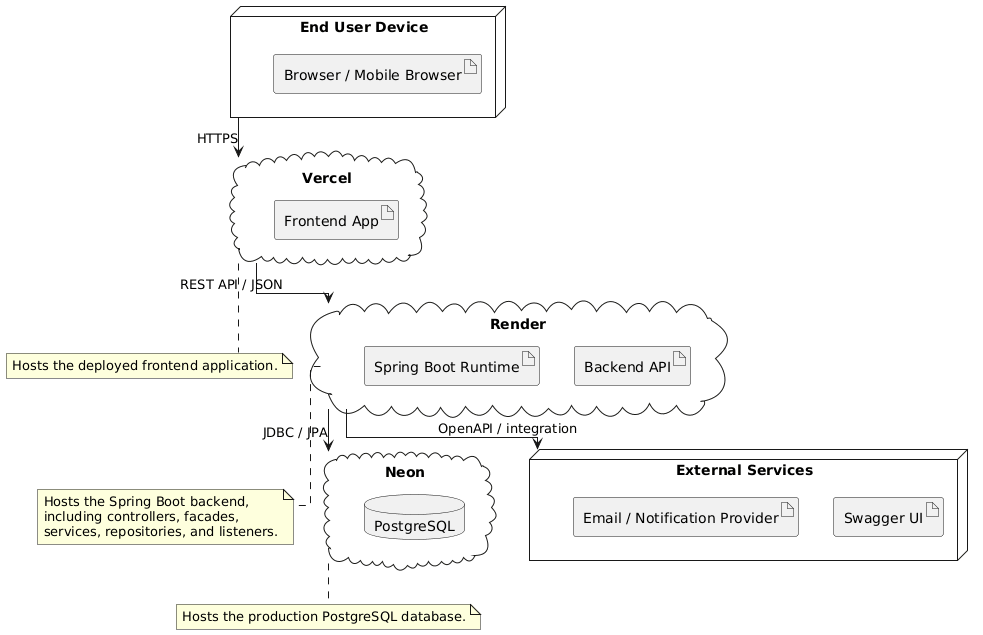
\includegraphics[width=0.95\linewidth]{image/4.3.2.png}
    \caption{Deployment Style của hệ thống}
    \label{fig:deployment-style}
\end{figure}

Sơ đồ Deployment Style mô tả cách hệ thống được triển khai trên các node và nền tảng hạ tầng thực tế.

\textbf{End User Device}:  
Người dùng truy cập hệ thống thông qua trình duyệt web hoặc mobile browser.

\textbf{Vercel}:  
Được sử dụng để triển khai frontend application của hệ thống.  
Frontend chịu trách nhiệm hiển thị giao diện người dùng và gửi request tới backend thông qua REST API.

\textbf{Render}:  
Được sử dụng để triển khai backend API chạy trên nền tảng Spring Boot Runtime.  
Backend bao gồm:
\begin{itemize}
    \item Controllers
    \item Facades
    \item Services
    \item Repositories
    \item Event listeners
\end{itemize}

\textbf{Neon}:  
Được sử dụng để triển khai cơ sở dữ liệu PostgreSQL trên cloud nhằm lưu trữ dữ liệu nghiệp vụ của hệ thống.

\textbf{External Services}:  
Bao gồm các dịch vụ tích hợp bên ngoài như:
\begin{itemize}
    \item Swagger UI phục vụ kiểm thử và tài liệu hóa API.
    \item Email / Notification Provider phục vụ gửi thông báo hệ thống.
\end{itemize}

\textbf{Luồng triển khai}:  
Người dùng truy cập frontend trên Vercel thông qua HTTPS, frontend gửi REST API request tới backend trên Render, sau đó backend tương tác với PostgreSQL trên Neon thông qua JDBC/JPA.

\vspace{0.5cm}

\subsubsection{Work Assignment Style}

% \begin{figure}[H]
%     \centering
%     \includegraphics[width=0.95\linewidth]{image/work-assignment-style.png}
%     \caption{Work Assignment Style của hệ thống}
%     \label{fig:work-assignment-style}
% \end{figure}

Work Assignment Style mô tả việc phân bổ trách nhiệm phát triển các module và nhiệm vụ trong hệ thống cho các nhóm phát triển tương ứng.

Hệ thống được phát triển thông qua nhiều nhóm khác nhau bao gồm:
\begin{itemize}
    \item Backend Team
    \item Frontend Team
    \item QA Team
    \item DevOps Team
\end{itemize}

Các nhiệm vụ chính của dự án bao gồm:
\begin{itemize}
    \item Requirements Analysis
    \item Architecture Design
    \item Auth Module
    \item Menu Module
    \item Order Module
    \item Kitchen Module
    \item Inventory Module
    \item Frontend Dashboard
    \item Integration Testing
    \item Deployment \& Monitoring
\end{itemize}

Mỗi task được phân công:
\begin{itemize}
    \item Team chịu trách nhiệm chính.
    \item Team hỗ trợ.
    \item Thời gian thực hiện.
    \item Module phụ thuộc.
    \item Deliverables đầu ra.
    \item Trạng thái thực hiện.
    \item Assignee chịu trách nhiệm trực tiếp.
\end{itemize}

Ngoài ra, Work Assignment Style còn sử dụng Gantt Chart để mô tả timeline phát triển hệ thống từ tuần 1 đến tuần 8.  
Gantt Chart giúp thể hiện:
\begin{itemize}
    \item Trình tự thực hiện các task.
    \item Quan hệ phụ thuộc giữa các module.
    \item Phân bổ thời gian cho từng nhóm phát triển.
    \item Tiến độ tổng thể của dự án.
\end{itemize}

Thông qua Work Assignment Style, nhóm phát triển có thể dễ dàng quản lý tài nguyên, phân chia trách nhiệm và theo dõi tiến độ thực hiện của toàn bộ hệ thống.

